\subsection{Results}

\subsubsection{Infrared-collinear safety}
The jet mass spectrum can be used to check for IRC safety.
For each configuration of the clustering algorithm we expect an IRC safe algorithm to give the 
same jet mass spectrum for both LO and NLO datasets.
Changes in the mass spectrum indicate sensitivity to the soft and collinear radiation that
has been included at NLO.


\begin{figure}[htp]
    \includegraphics[width=\textwidth]{graphics/IRC_singles}
    \caption{Spectrums for jet properties created with LO and NLO datasets.
             The columns from left to right are; the jet mass (which would be IRC sensitive),
             the jet \(p_T\) (which would also be IRC sensitive),
             the barrel angle of the jets and the rapidity of the jets.
             Algorithms where configured (i.e. settings of \stoppingdeltar{} chosen)
             to give sensible results on
             this dataset, therefore may not represent worst case scenarios.
             Looking at these graphs it is not immediatly clear that the Generalised KT
             algorithm is IRC safe and the Iterative Cone algorithm is unsafe, 
         much less what the status of Spectral clustering is.}
%    \begin{minipage}[c]{0.47\textwidth}
%        \includegraphics[width=\textwidth]{graphics/worst_antikt_histOnly.png}
%        \caption{The jet mass spectrums of the Generalised KT algorithms that
%                 differed the most between LO and NLO datasets.
%                 This algorithm had a \(p_T\) exponent of \(1.\),
%                 (so the form of the \(p_T\) factor is between Cambridge-Aachen and KT),
%                 it used taxi-cab distances in physical space
%                 and \(\stoppingdeltar{} = 1.5\).
%                 Little divergence can be seen.
%        }
%    \end{minipage}\hfill
%    \begin{minipage}[c]{0.45\textwidth}
%        \includegraphics[width=\textwidth]{graphics/worst_spectral_histOnly.png}
%        \caption{The jet mass spectrums of the Spectral algorithms that
%                 differed the most between LO and NLO datasets.
%                 This algorithm calculated affinities as
%                 \(a_{i,j} = \text{exp}\left((\delta \phi_{i, j}^2 + \delta y_{i, j}^2)/0.3\right)\).
%                 The Laplacian is symmetric and 
%                 as many eigenvector as can be found are used which are
%                 normalised as \(x_{i,\text{normed}} = x_i/\lambda_i^{1.8}\).
%                 There is no use of \(p_T\) and \(\stoppingdeltar{} = 1.3\).
%                 Little divergence can be seen.
%        }\label{fig:spectralircexample}
%    \end{minipage}
%    \begin{minipage}[c]{0.48\textwidth}
%        \includegraphics[width=\textwidth]{graphics/worst_iterativecone_histonly.png}
%        \caption{The jet mass spectrums of the Iterative Cone algorithms that
%                 differed the most between LO and NLO datasets.
%                 This algorithm had a \(p_T\) exponent of \(1.\),
%                 (so the form of the \(p_T\) factor is between Cambridge-Aachen and KT),
%                 it used taxi-cab distances in physical space
%                 and \(\stoppingdeltar{} = 0.34\).
%                 Some divergence is seen, particularly at low mass.
%        }\label{fig:iterconeircexample}
%    \end{minipage}
\end{figure}    

%
%\begin{figure}[htp]
%    \includegraphics[width=1.\textwidth]{graphics/same_bin_size_worst_all_jets.png}
%    \caption{Same plots as previous, but with the same x-axis.
%        Last bin is overflow bin.
%    }
%\end{figure}    
%

As described in section~\ref{sec:IRCmethod} this can be systematically compared for many hyperparameter configurations by calculating a Jensen-Shannon
score for each LO-NLO pair of jet mass spectrums.
If the Jensen-Shannon metric is low, then the two distributions are similar and appear IRC safe.
This can be seen in fig~\ref{fig:unnormedJS}.

This comparison is slightly complicated by the fact that we must use a completely different set of events,
so if a clustering algorithm tends to produce more noisy mass spectrums (on varied events)
anyway it will increase the gap between the NLO and the LO datasets even if no IRC sensitivity is present.
Again, as described in section~\ref{sec:IRCmethod} the influence of this noise can be investigated.
This can be seen in fig~\ref{fig:jensenshannon}.

From both these figures it is clear that spectral clustering is IRC safe.
This is not unexpected, as the inputs to spectral clustering
are the same as for the Cambridge-Aachen algorithm, 
which is itself IRC safe.
However it is good to have a verification in data.

\begin{figure}[htp]
    \begin{minipage}[c]{0.6\textwidth}
    \includegraphics[width=1.\textwidth]{graphics/JensenShannon_unnormed.png}
    \end{minipage}\hfill
    \begin{minipage}[c]{0.35\textwidth}
    \caption{Here is the raw distribution of Jensen-Shannon scores.
        Each count is a Jenson Shannon score between a probability density of jet mass from LO data and
        from NLO data, as described in section~\ref{sec:IRCmethod}.
        Counts at low values indicate insensitivity to IRC difference between the LO and NLO data,
        thus IRC safety.
        Spectral methods produce Jensen Shannon scores similar to Generalised-KT
        methods. Only Iterative cone produced high Jenson shannon scores indicating changes
        between the LO and NLO spectrums.
     }\label{fig:unnormedJS}
    \end{minipage}
\end{figure}    
\begin{figure}[htp]
    \begin{minipage}[c]{0.6\textwidth}
    \includegraphics[width=1.\textwidth]{graphics/JensenShannon.png}
    \end{minipage}\hfill
    \begin{minipage}[c]{0.35\textwidth}
    \caption{Here is the distribution of subsampled Jensen-Shannon scores.
        Each count is a subsampled Jenson Shannon score between a probability density of jet mass from LO data and
        from NLO data, as described in section~\ref{sec:IRCmethod}.
        Counts at low values indicate insensitivity to IRC difference between the LO and NLO data,
        thus IRC safety.
        Spectral methods produce Jensen Shannon scores similar to Generalised-KT
        methods. Only Iterative cone produced high Jenson shannon scores indicating changes
        between the LO and NLO spectrums.
        From this it is clear that spectral methods are IRC safe,
        and that the volume of data used to produce this figure and figure~\ref{fig:unnormedJS},
        was sufficient to mitigate the effects of noise.
    }\label{fig:jensenshannon}
    \end{minipage}
\end{figure}    


%I have yet to find a definition of relative PT that makes sense in the context of jets,
%so I haven't been able to add that metric.
\FloatBarrier{}
\subsubsection{Mass peak reconstruction}
In this section Anti-KT algorithms, with jet radius \(\stoppingdeltar{} = 0.4\) and \(\stoppingdeltar{} = 0.8\)
are compared to the spectral clustering algorithm specified in section~\ref{sec:spectralmethodparam}.


Firstly, jet multiplicities, that is number of jets found per event are given.
These can be seen for three data samples in fig~\ref{fig:multiplicity}


\begin{figure}[htp]
    \begin{minipage}[c]{0.32\textwidth}
        \includegraphics[width=\textwidth]{graphics/multiplicity/light_higgs.png}
    \end{minipage}\hfill
    \begin{minipage}[c]{0.33\textwidth}
        \includegraphics[width=\textwidth]{graphics/multiplicity/heavy_higgs.png}
    \end{minipage}\hfill
    \begin{minipage}[c]{0.29\textwidth}
        \includegraphics[width=\textwidth]{graphics/multiplicity/tt_bar.png}
    \end{minipage}\hfill
    \caption{Jet multiplicities for spectral clustering, on three data samples.
    }\label{fig:multiplicity}
\end{figure}    



As the data is simulated, it is possible to compare the performance of clustering algorithms to Monte Carlo truth.
Each higgs cascade event contains 4 \bthing{quarks} and for each of them it is possible to identify the particle into which they decayed, as a subset of the particles in the final state.
Henceforth the detectable decay products of the \bthing{quark} will be called the descendants of the \bthing{quark}.
For two reasons it is not possible for this clustering algorithm to gather all the descendants
of each \bthing{quark} into one jet:
firstly, not all the descendants make the \(p_T\) and \(\eta\) cuts, so some are discarded before clustering;
secondly, the descendants of the \bthing{quarks} in an event are not mutually exclusive, due to interactions during hadronisation the quarks share descendants, and our clustering algorithm does produce exclusive clusters.

Combining these factors with the \(p_T\) cuts, almost \(2/3\) of the objects could be reconstructed in theory.

Knowing the parts of the final state that are descended from each \bthing{quark} creates a clear
allocation of jets to quarks.
For each quark, the jet that contains the greatest mass in descendent particles is tagged to represent that quark.

Mass peaks can the be constructed from the tagged jets, using all the particles in the jet,
both descendant of the quarks and background.
The mass peaks for the Spectral configuration described and anti-kt 
with \(\stoppingdeltar{} = 0.8, 0.4\) are given for comparison.
In figure~\ref{fig:best_correct_h_allocation} three selections are plotted; firstly only events where some trace of all 4 \bthing{quarks} is found
are plotted with the mass of the descendants of the heavy Higgs in the background.
Then the two light Higgs in each event are sorted by the mass of their descendants,
in effect they are ranked by how well they were picked up by the detector.
The mass of the light descendants is plotting in the background and over
that the mass of the associated jets in each event is shown.




\begin{figure}[htp]
    \includegraphics[width=1.\textwidth]{graphics/mass_peaks/light_long_correct_frequency.png}
    \caption{Starting with the plot on the far right, the jet mass of events where
        some descendants from all 4 \bthing{quarks} were found is plotted over
        the total mass of all descendants.
        The plot on the left takes the light Higgs whose descendants have the greatest mass in each event.
        The mass of these descendants is plotted in grey, and over this
        the masses of the jets in each event that correspond to this better observed Higgs
        are shown.
        That is, the tags in each event that have been produced by the better observed light Higgs
        are allocated to jets, and only the mass of these jets is tabulated - thus
        a good cluster will have obtained the mass of the light Higgs descendants.
        Finally, in the centre, the light Higgs whose descendants have less mass is shown along with
        the corresponding jets.
    }\label{fig:best_correct_h_allocation}
\end{figure}    



\begin{figure}[htp]
    \includegraphics[width=1.\textwidth]{graphics/mass_peaks/heavy_long_correct_frequency.png}
    \caption{Starting with the plot on the far right, the jet mass of events where
        some descendants from all 4 \bthing{quarks} were found is plotted over
        the total mass of all descendants.
        The plot on the left takes the light Higgs whose descendants have the greatest mass in each event.
        The mass of these descendants is plotted in grey, and over this
        the masses of the jets in each event that correspond to this better observed Higgs
        are shown.
        That is, the tags in each event that have been produced by the better observed light Higgs
        are allocated to jets, and only the mass of these jets is tabulated - thus
        a good cluster will have obtained the mass of the light Higgs descendants.
        Finally, in the centre, the light Higgs whose descendants have less mass is shown along with
        the corresponding jets.
    }
\end{figure}    


\begin{figure}[htp]
    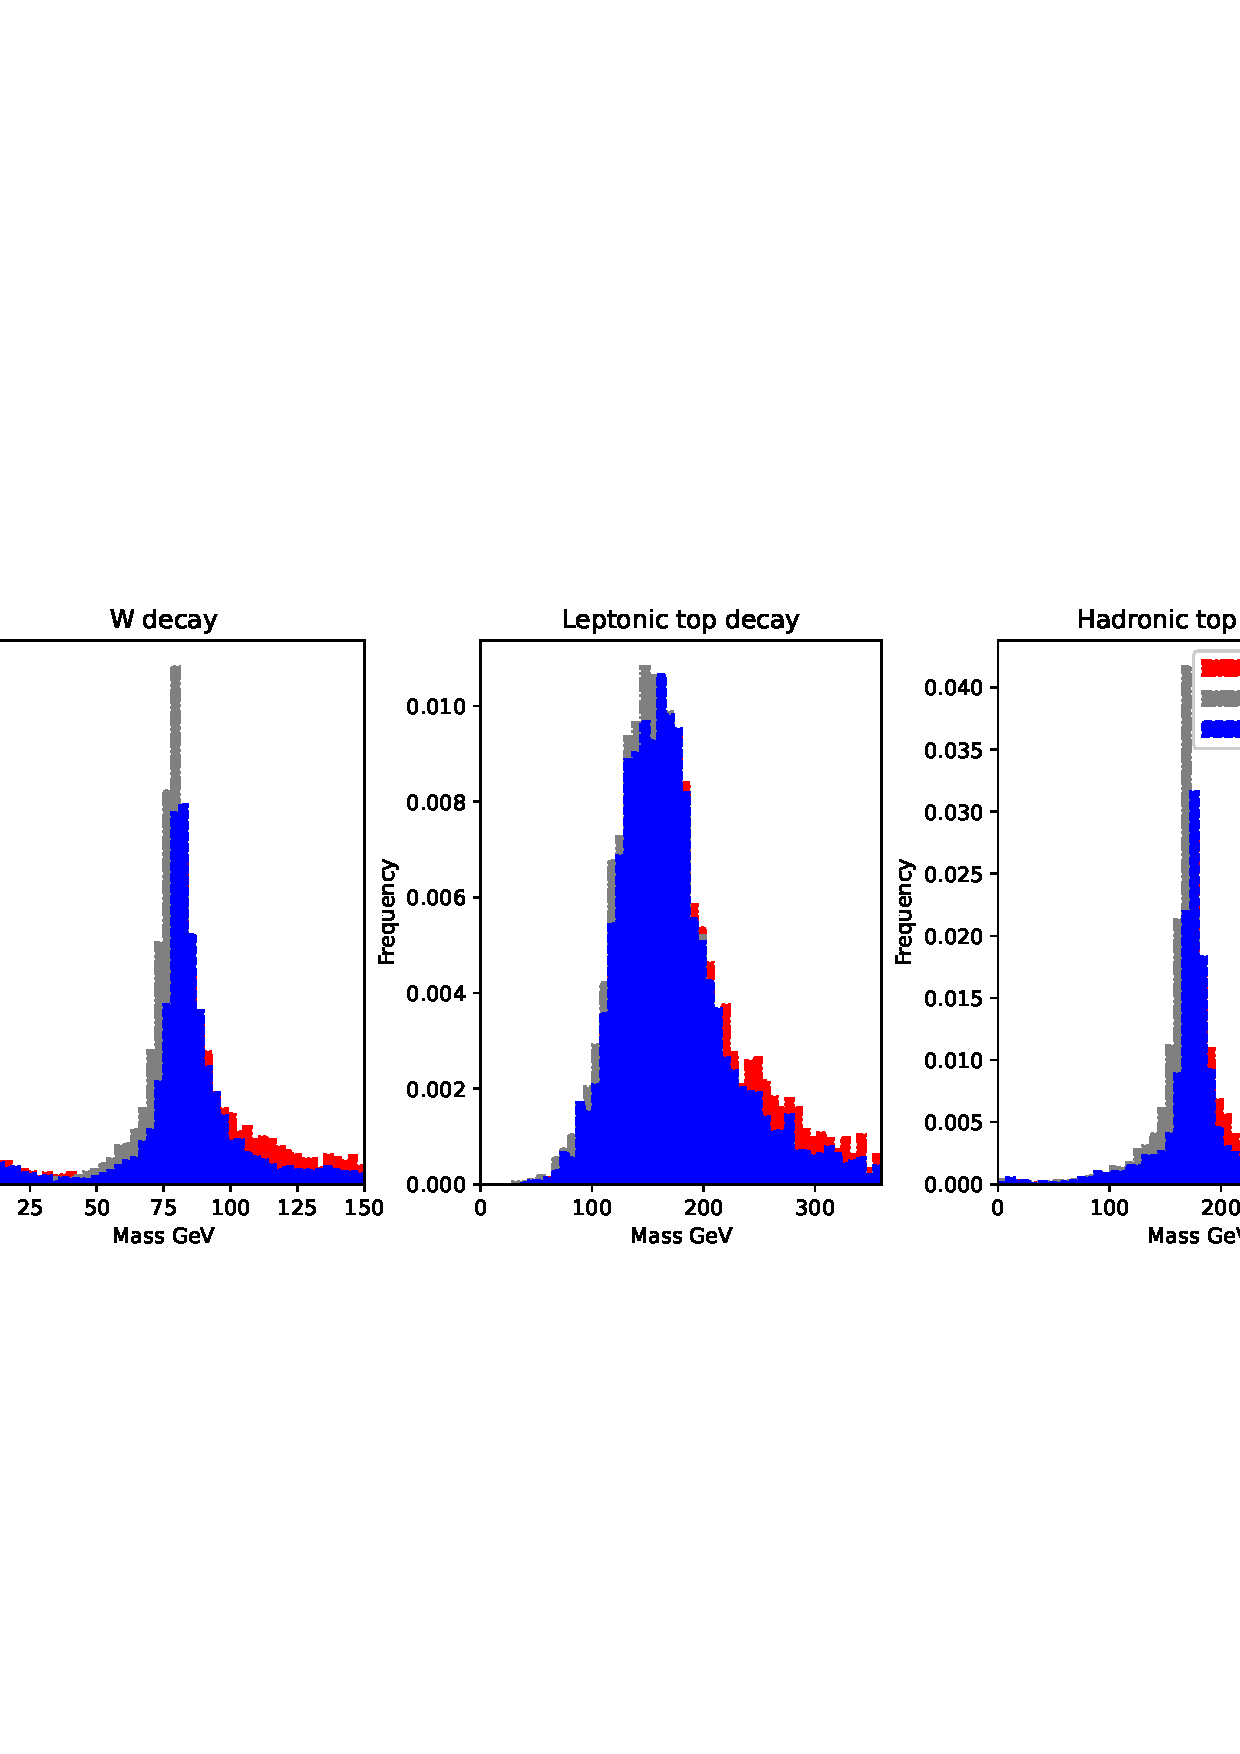
\includegraphics[width=1.\textwidth]{graphics/mass_peaks/top_long_correct_frequency.png}
    \caption{
        Both plots show the mass of a top, which decays to a \bthing{quark} and a $W$.
        The contribution of the \bthing{quark} is a reconstruction using spectral clustering,
        and the contribution of the $W$ is taken from Monte Carlo.
        Each event contains a \(t\)-\(\bar{t}\) pair.
        The plot on the left shows the top whose descendants have the greatest mass in each event.
        The mass of these descendants is plotted in grey, and over this
        the masses of the jets in each event that correspond to this better observed Higgs
        are shown.
        That is, the tags in each event that have been produced by the better observed light Higgs
        are allocated to jets, and only the mass of these jets is tabulated - thus
        a good cluster will have obtained the mass of the light Higgs descendants.
        Finally, on the right is the top whose descendants have less mass is shown along with
        the corresponding jets.
    }
\end{figure}    

%\begin{figure}[htp]
%    \includegraphics[width=1.\textwidth]{graphics/show2_40.png}
%    \caption{Mass peaks for the light higgs cascade;
%    \(p^+ p^+ \rightarrow H_{125\text{GeV}} \rightarrow h_{40\text{GeV}} h_{40\text{GeV}} \rightarrow \beau \bbar \beau \bbar\).
%        Jets are required to have at least 2 particles and \(15\) GeV \(p_T\).
%        The left hand peak is the mass of all jets in events where 4 jets are reconstructed.
%        The central plot is the mass of the dijet pair closest to \(40\) GeV,
%        the right hand plot is the remaining dijet pair.
%    }
%\end{figure}    
%
%\begin{figure}[htp]
%    \includegraphics[width=1.\textwidth]{graphics/show2_125.png}
%    \caption{Mass peaks for the heavy higgs cascade,
%    \(p^+ p^+ \rightarrow H_{500\text{GeV}} \rightarrow h_{120\text{GeV}} h_{120\text{GeV}} \rightarrow \beau \bbar \beau \bbar\).
%        Jets are required to have at least 2 particles and \(30\) GeV \(p_T\).
%        The left hand peak is the mass of all jets in events where 4 jets are reconstructed.
%        The central plot is the mass of the dijet pair closest to \(125\) GeV,
%        the right hand plot is the remaining dijet pair.
%    }
%\end{figure}    



%There are also some values that can be given to compare these two jets;
%\begin{enumerate}
%    \item Quality fraction~\cite{JetQuality2008}. A window on the reconstructed masses,
%        size proportional to the root of mass of the object to be reconstructed,
%        across the data. The total number of generated objects (in this dataset 2000)
%        is divided by the maximum number of reconstructed objects in the window,
%        and this is the quality width.
%        
%        \[\text{Anti-KT (\(\stoppingdeltar{} = 0.8\)) Quality Fraction} = 1.33\text{GeV}\]
%        \[\text{Spectral Quality Fraction} = 1.33\text{GeV}\]
%    \item Quality width~\cite{JetQuality2008}. A required fraction of the generated objects,
%        in this case \(0.15\) is selected.
%        The smallest mass window that can capture this fraction is determined.
%        
%        \[\text{Anti-KT (\(\stoppingdeltar{} = 0.8\)) Quality Width} = 0.00141\text{GeV}\]
%        \[\text{Spectral Quality Width} = 0.000129\text{GeV}\]
%    \item Signal mass lost. The mass of the particles descendent from the light higgs
%        that are visible on the barrel is compared to the mass of the subset of those
%        particles that was found in the jet. The higher the number the more
%        signal particles are missing from the jet.
%        \[\text{Anti-KT (\(\stoppingdeltar{} = 0.8\)) Signal mass lost} = 1.80\text{GeV}\]
%        \[\text{Spectral Signal mass lost} = 2.17\text{GeV}\]
%    \item Background contamination. The mass of all the background objects,
%        either from the wrong higgs or from gluons, found in jets.
%        The higher the number the more the jets are tending to include too many particles.
%        \[\text{Anti-KT (\(\stoppingdeltar{} = 0.8\)) Background contamination} = 1.92\text{GeV}\]
%        \[\text{Spectral Background contamination} = 1.56\text{GeV}\]
%\end{enumerate}
%
